\documentclass[11pt, oneside]{article} 
\usepackage{geometry}
\geometry{letterpaper} 
\usepackage{graphicx}
	
\usepackage{amssymb}
\usepackage{amsmath}
\usepackage{parskip}
\usepackage{color}
\usepackage{hyperref}

\graphicspath{{/Users/telliott_admin/Dropbox/Tex/png/}}
% \begin{center} 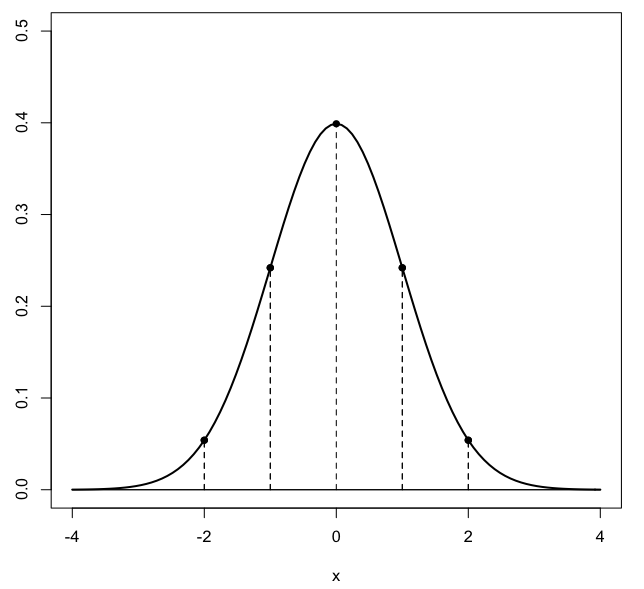
\includegraphics [scale=0.4] {gauss3.png} \end{center}

\title{Pentagons}
\date{}

\begin{document}
\maketitle
\Large
In this short write-up we explore some properties of a regular pentagon.  First, draw all of the internal chords of the figure and label some angles.  It will turn out that all the angles have one of only three different measures in the figure, but for now we label them as $a$-$d$.
\begin{center} 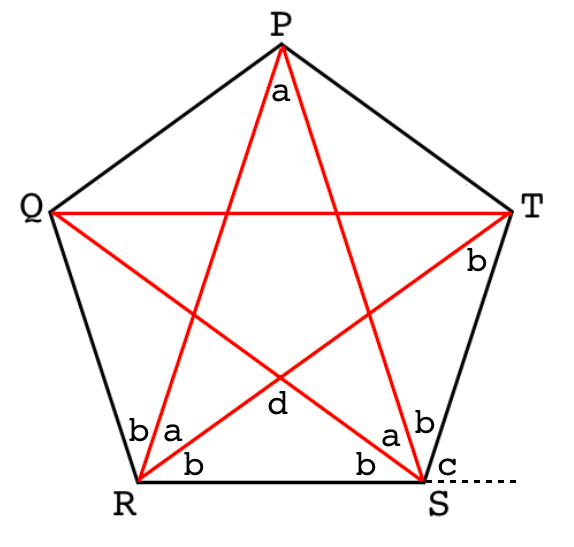
\includegraphics [scale=0.35] {pent_chords.png} \end{center}

One way to start thinkgin about the angles is to imagine that we walk along $RS$ and then make a left-turn at $S$, to face $T$.  The angle through which we turn is $c$.  In going around the whole perimeter to return to R (and face horizontally again) we turn 5 times.  Hence $5c = 2 \pi$
or
\[ c = 2 \cdot \frac{\pi}{5} \]
It will turn out that all the angles are multiples of $\pi/5$.

Next, observe that the angles labeled $a$ are equal, by the five-fold rotational symmetry of the figure.  There are 5 such angles in total.

The measure of the whole angle at each vertex of the pentagon is $b + a + b$.  The equality of $b$ on the left and right sides of $a$ follows, again, from rotational symmetry.

The vertex angle is $b + a + b$, that angle plus $c$ is
\[ b + a + b + c = \pi \]
and since $c = 2 \cdot \pi/5$, we compute that $b + a + b = 3 \cdot \pi/5$.

Now consider $\triangle RST$.  The sum of the angles in this triangle is 
\[ b + b + a + b + b = \pi \]
Using the previous computation for $b + a + b$, we easily find that $2b = 2 \cdot \pi/5$ and thus $b = \pi/5$.  Reusing the result for $b + a + b = 3 \cdot \pi/5$, we find that $a = b = \pi/5$.

\begin{center} 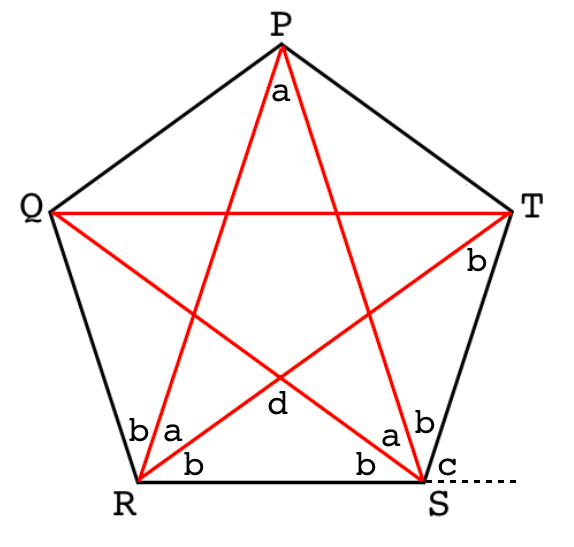
\includegraphics [scale=0.35] {pent_chords.png} \end{center}

Comparing $\triangle RST$ to the small triangle with $R$ and $S$ as vertices (or simply computing with the value $b = \pi/5$), we see that $d$ is equal to $3 \cdot \pi/5$.  Therefore the inner pentagon is also a regular pentagon, which we could have deduced from the rotational symmetry alone.

Now observe the angle that $QT$ makes with $ST$.  This angle is equal to $c$ (that is, $2 \cdot \pi/5$), and therefore these are alternate interior angles of two parallel lines.  Thus $QT$ is parallel to $RS$.  (Or simply add the included angles $a + b + b + a + b = \pi$).

One can draw two types of isosceles triangles using the chords and sides of the pentagon.  One is short and fat, the other, tall and skinny.  The first class have base angles equal to $2 \cdot \pi/5$ and the second, base angles equal to $\pi/5$.  Here are three examples of tall and skinny:
\begin{center} 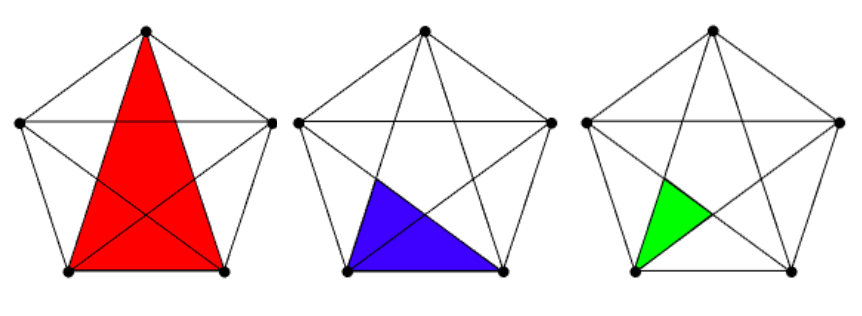
\includegraphics [scale=0.4] {three_triangles.png} \end{center}

If we take the side length of the pentagon to be 1, then the long side length of the red triangle is $1$ plus some other value, call that $x$.  $x$ is also the length of the short side or base for the blue triangle.  We use the fact that red and blue are similar and form the ratio $\phi$ of the long side to the base (red on the left, blue on the right):
\[ \phi = \frac{1 + x}{1} = \frac{1}{x} \]
Rearrange:
\[ x^2 + x - 1 = 0 \]
\[ x = \frac{-1 \pm \sqrt{1 + 4}}{2} \]
Of course $\phi$ is the golden ratio where we have taken the positive branch of the square root:
\[ \phi = 1 + x = \frac{1 + \sqrt{5}}{2} \]

\end{document}